\section{Keymaps alternatives}

% Troll disclaimer~: on ne s’intéresse qu’aux keymaps qui peuvent intéresser la
% majorité des épitéens…

\begin{frame}{Généralités}
    \begin{itemize}
        \item «~X n’est pas adapté au code, c’est plus facile en QWERTY~» \pause
            \begin{itemize}
                \item Les avis divergent fortement, faites-vous votre propre
                  avis. \pause

                \item Le code est généralement composé de mots anglais, plus
                  des commentaires.
            \end{itemize}
            \pause

        \item Keymap adaptée au français~: toujours plus adaptée à
          l’anglais qu’un QWERTY ou AZERTY
          % Ce sont deux langues d’origine plus ou moins latines, assez
          % similaires.
    \end{itemize}
\end{frame}



\subsection{Canadien multiligue}

\begin{frame}{Canadien multilingue}
    \centering
    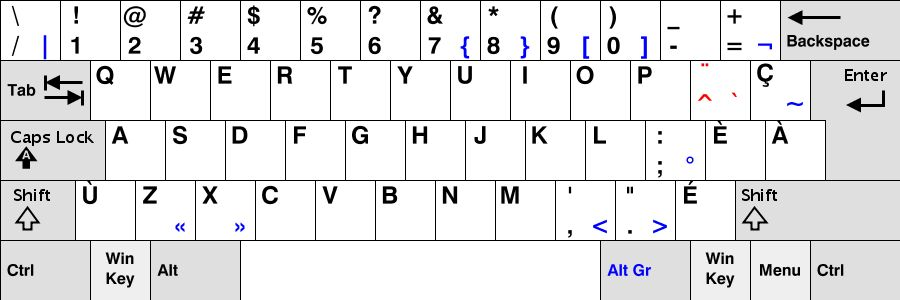
\includegraphics[width=\textwidth]{images/ca-multi.jpg}
    \pause

    \begin{itemize}
        \item Très proche du QWERTY \pause

        \item Accès direct à la plupart des signes typographiques français
          courants (il en manque certains comme «~…~») \pause
        % Lettres accentuées (et «~ç~») en accès direct, ainsi que les
        % majuscules avec Shift, espace insécable

        \item Accès direct aux chiffres (pas besoin de Shift) \pause

        \item Délimiteurs par paire («~[~» à côté de «~]~», idem pour «~(~»,
          etc.)
    \end{itemize}
\end{frame}



\subsection{US International}

\begin{frame}{US International}
    \centering
    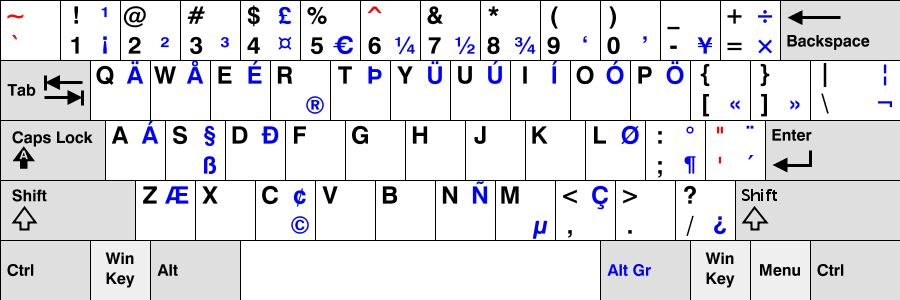
\includegraphics[width=\textwidth]{images/us-intl.jpg}
    \pause

    \begin{itemize}
	\item Quasiment identique au QWERTY \pause

        \item Rajout de quelques caractères supplémentaires (accès~: touches mortes ou Alt~Gr)
    \end{itemize}
\end{frame}



\subsection{Dvorak — DSK}

\begin{frame}{Le Dvorak}
    \centering
    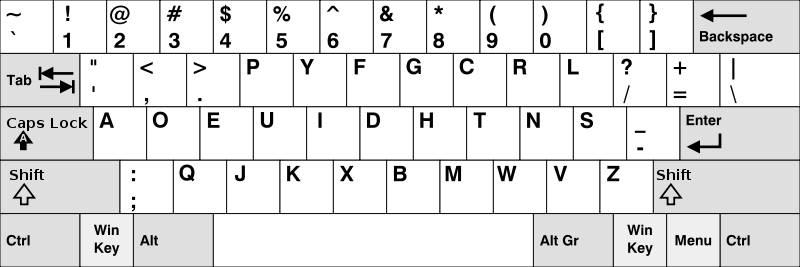
\includegraphics[height=90pt]{images/dvorak.png}
    \pause

    \begin{itemize}
	\item Le dvorak, ou clavier américain simplifié (DSK). \pause

	\item Conçu par la méthode Dvorak~: en étudiant les langues
          cibles. \pause

	\item Créé dans les années 1930 par August Dvorak et William Dealey.
    \end{itemize}
\end{frame}

\begin{frame}{Le DSK}
    \begin{itemize}
	\item Clavier inadaptable pour d’autre langues. \pause

	\item Quelques unes pour le français (Dvorak-fr, fr-Dvorak,
          Dvorak-international). \pause

	\item Une seule tient la route~: le Bépo.
    \end{itemize}
\end{frame}



\subsection{Bépo}

\begin{frame}{Caractéristiques}
    % Ne pas oublier de parler de la création du Bépo (communauté sur Internet,
    % méthode Dvorak et donc étude statistique, améliorations successives, et
    % version maintenant stable)

    \centering
    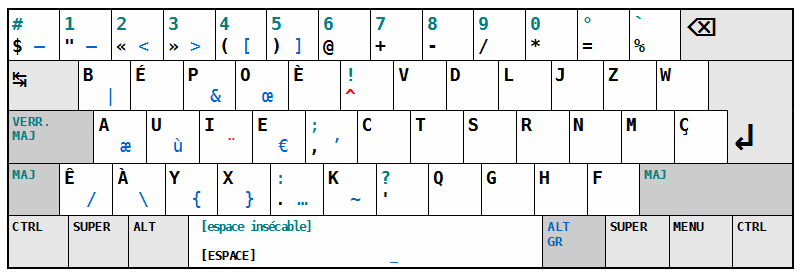
\includegraphics[width=\textwidth]{images/bepo-simple.png}
    \pause

    \begin{itemize}
	\item 70~\% des lettres nécessaires sont sur la ligne centrale~: moins
          de mouvement pour les mains. \pause

        \item Disposition telle qu’il y ait le plus d’alternance possible entre
          les deux mains. \pause

	\item S’apprend très facilement.
    \end{itemize}
\end{frame}

\begin{frame}{Carte complète}
    \centering
    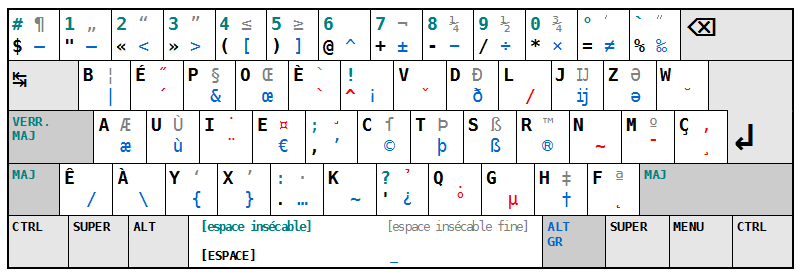
\includegraphics[width=\textwidth]{images/bepo-complete.png}
    \pause

    \begin{itemize}
        \item Le jeu de caractères facilement accessible est \emph{très}
          riche. \pause

        \item Il est particulièrement adapté au français~: lettres et signes
          typographiques.
    \end{itemize}
\end{frame}
